%
% Copyright (C) 2011 Agostino De Marco
%                    <agostino dot demarco at unina dot it>
%                    Roberto Giacomelli
%                    <giaconet dot mailbox at gmail dot com>
%
%    This work may be distributed and/or modified under the
%    conditions of the LaTeX Project Public License, either
%    version 1.3 of this license or any later version.
%    The latest version of this license is in
%    http://www.latex-project.org/lppl.txt and version 1.3
%    or later is part of all distributions of LaTeX version
%    2005/12/01 or later.
%
% This work has the LPPL maintenance status `maintained'.
% 
% The Current Maintainer of this work are Agostino De Marco
% and Roberto Giacomelli
%
\documentclass{standalone}
\usepackage{lmodern}
\usepackage{amsmath,fixmath}
\usepackage{relsize}
\usepackage{pgfplots}
\usetikzlibrary{intersections}

\pgfkeys{/pgfplots/linelabel/.style args={#1:#2:#3}{name path global=labelpath,execute at end plot={
\path [name path global = labelpositionline]
(rel axis cs:#1,0) --
(rel axis cs:#1,1);
\draw [help lines,text=black,inner sep=0pt,name intersections={of=labelpath and labelpositionline}] (intersection-1) -- +(#2) node [label={#3}] {};},
}}

\pgfplotsset{%
    every axis legend/.append style={
        cells={anchor=west},%
        fill=gray!10,
        font=\relsize{1},
        at={(0.97,0.03)},
        anchor=south east,thin,draw=none
        }
}

\pgfplotsset{every axis title/.append style={font=\relsize{1}}}
\pgfplotsset{every axis/.append style={font=\relsize{0}}}
\pgfkeys{/pgf/number format/.cd,fixed,precision=2,use comma}
\pgfplotsset{
    every axis x label/.append style={
                font=\relsize{1},
                yshift=0pt,xshift=0em}
}
\pgfplotsset{
    every axis y label/.append style={
                font=\relsize{2},
                rotate=-90, % -90,
                xshift=-0.0em, % -0.2em,
                yshift=0.0em, % 0.5em
    }
}
\pgfplotsset{
    every axis/.append style={
        thick,% thick
        tick style={thick}} % semithick
}

\tikzstyle{every pin}=[fill=white,draw=none,font=\relsize{2}]

\begin{document}
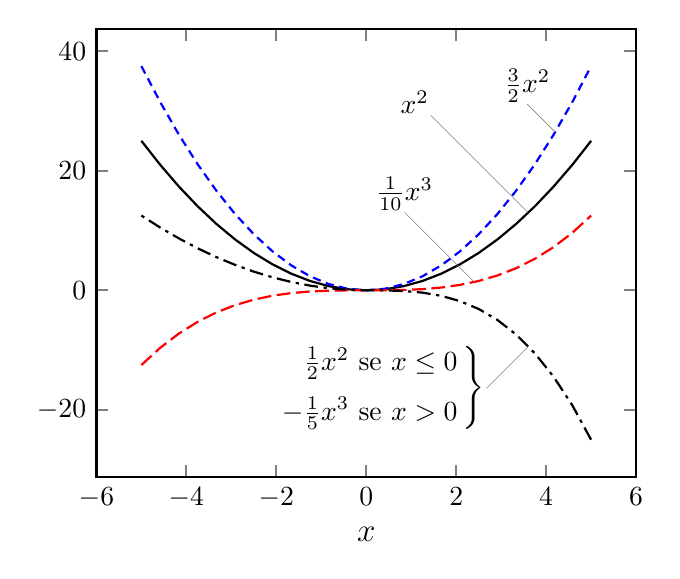
\begin{tikzpicture}
\begin{axis}[
xlabel={$x$}
]

\addplot [thick, 
    linelabel=0.8:{135:1.75cm}:
        {[black]above left:$x^2$}] {x^2};
\addplot [thick, 
    blue,
    densely dashed,
    linelabel=0.85:{135:0.50cm}:
        $\frac{3}{2}x^2$] {1.5*x^2};
\addplot [thick, 
    red,
    dash pattern=on 5pt off 2pt,
    linelabel=0.7:{135:1.25cm}:
        $\frac{1}{10}x^3$] {0.1*x^3};

\addplot [thick, 
    dash pattern=on 1.2pt off 2pt on 5pt off 2pt,
    linelabel=0.80:{-135:0.75cm}:
        {left:
            $
                  \begin{array}{@{}r@{\ }l@{$\,$}}
                      \frac{1}{2}x^2 &\text{se }x\le 0\\[6pt]
                      -\frac{1}{5}x^3 &\text{se }x> 0
                  \end{array}\Biggr\}
            $
        }
    ]
    {(x<0)*0.5*x^2 + (x>0)*(-0.20*x^3)};

\end{axis}
\end{tikzpicture}
\end{document}